\question[10] Ordena los metales de menor (1) a mayor (5) precio; considera los datos de la tabla \ref{fig:SINMAT1_U3_AC72_IMG2}.
\begin{figure}[H]
    \centering
    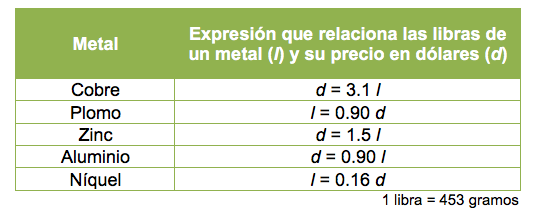
\includegraphics[width=0.6\textwidth]{../images/SINMAT1_U3_AC72_IMG2}
    \caption{Tabla de relaciones de precios en dolares algunos metales.}
    \label{fig:SINMAT1_U3_AC72_IMG2}
\end{figure}
\begin{parts}
    \part \fillin[5] Niquel
    \part \fillin[2] Plomo
    \part \fillin[4] Cobre
    \part \fillin[1] Aluminio
    \part \fillin[3] Zinc
\end{parts}


